%\section{Design-for-Testibility with }
\section{Constructing Design-for-Testability Biochip Architecture}\label{sec:dft_arch}

In this section, we explain the strategy and the implementation to generate an 
augmented biochip architecture and the corresponding test vectors.
%and the schedule of the application on the new architecture.

As observed in \figname~\ref{fig:multiPortSingPort}, a biochip with multiple
ports can obtain single-source single-meter testability by adding additional
DFT channels and valves.  In the proposed method, the locations of these
channels and valves are determined by mapping the input chip architecture to a
virtual connection grid, as shown in \figname~\ref{fig:fitintogrid}. In this
mapping, devices are assigned to nodes and channels to edges in the
grid, while keeping the original topology of the chip unchanged.  After this
mapping, the nodes and edges that have not been occupied in the connection
grid represent the possibilities where additional channels and valves can be
built. 
In the mapping in \figname~\ref{fig:fitintogrid}, valves need not to be mapped
to the nodes explicitly,
%included, 
because they are needed only at the inputs/outputs of devices and the crossing
points between channels and they are tested together with valves.
%automatically when channels are tested.

%. The testing vectors enable flow paths to
%test stuck-at-0 defects. If a path covers several segments of the
%transporation channels, the valve on them are tested automatically. For
%example, alougth the vavles on the test path P1 do not appear in the
%connection grid, a stuck-at-0 defect on them can still be detected because no
%pressue can be measured at the pressure meter.  Therefore, the channels need
%only to be inserted back after DFT channels are created.  

The 
%single-source single-meter 
testability of stuck-at-0 defects of a biochip requires that for each valve or
channel, there is a path from the single pressure source to the single
pressure meter.  In the proposed method, we use this requirement to identify
the locations of new channels and valves. Afterwards, test cuts are
generated from the augmented architecture to test stuck-at-1 defects.

For a given biochip architecture, there might be multiple possibilities to add
channels and valves to implement the single-source single meter testability.
In the following, a feasible solution of this testability problem is called a
\textit{DFT configuration}. In the proposed method, we identify the DFT
configurations using Integer Linear Programming (ILP) programming.

Assume there is a path $p_r$ between nodes $n_{s}$ and $n_{t}$, which
represent the locations of the external ports 
%of the given biochip mapped onto 
on the connection grid. We use a 0-1 variable $e_{j,r}$ to represent whether
the edge $e_j$ in the connection grid is on the path $p_r$, and the 0-1
variable $n_{i,r}$ to represent whether the node $n_i$ is on the path $p_r$.
For nodes $n_{s,r}$ and $n_{t,r}$, only one of the four edges incident to it 
%to each of them 
can be covered by the path $p_r$.  
%a node $n_i$ on a test path between 
At each other node $n_i$ on the path, exactly two edges incident to it are
covered.  Accordingly, we can construct the path with the following
constraints,
\begin{align}\label{eq:path_construct} 
% \sum_{e_j\in E_s}e_{j,r}=\sum_{e_j\in E_t}e_{j,r}=1,\quad 
 \sum_{e_j\in E_i}e_{j,r} = 2n_{i,r} ,\quad \forall n_i\in N, n_i \ne n_{s}, n_{t}\\ 
  \sum_{e_j\in E_i}e_{j,r} = 1, \quad  \forall n_i = n_{s}, n_{t}
\end{align}
where 
%$E_s$, $E_t$ and 
$E_i$ is the set of edges incident to the node 
$n_i$ and $N$ is the set
of all the nodes in the connection grid.

\begin{figure}
\figurefontsize
\centering
%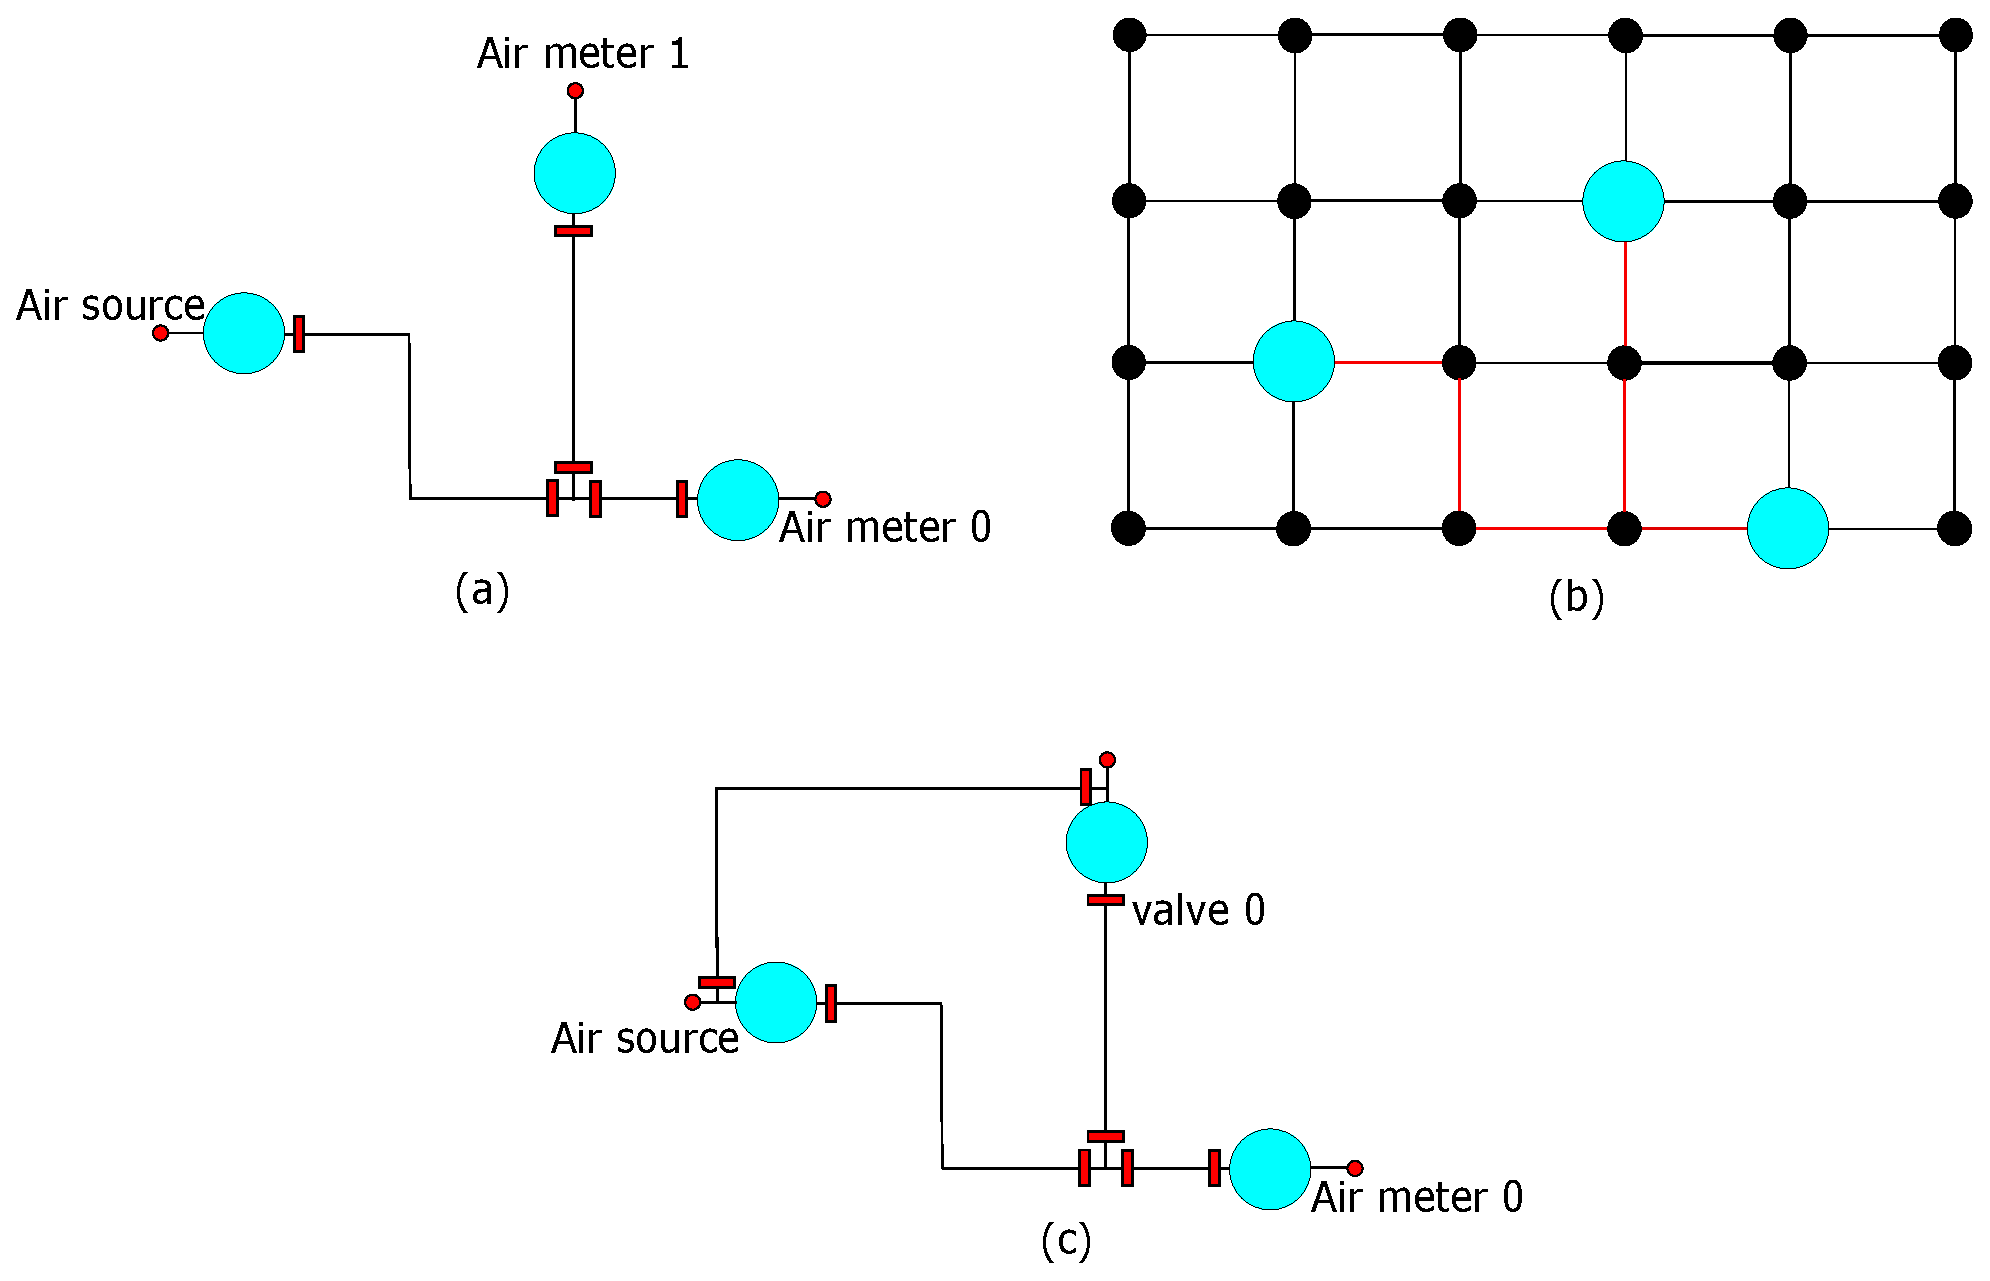
\includegraphics[width=3.50in,height=2.2in]{Fig/fitintogrid2.eps}
\input{Fig/grid.pdf_tex}
\caption{Mapping a biochip onto a virtual connection grid.}
%(a) Origin biochip. (b) Connection grid after mapping. Thick edges 
%represent the edges occupied by the original channels.}
%(c) Design-for-test architecture}
\label{fig:fitintogrid}
\end{figure}


Since the channel segments occupied by the original chip must appear in the new
architecture, the constraints for these edges can be written as
\begin{equation}\label{eq:edge_cover}
\sum_{p_r\in P} e_{j,r}\ge 1,\quad \forall e_j\in E_{o} 
\end{equation}
where $P$ is the set of all test paths; $E_{o}$ is the set 
of edges occupied by the original channels in the connection grid.

When generating the DFT architecture of the chip, we minimize the number of
added channels.
We use a 0-1 variable $s_j$ to represent whether the edge $e_j$ in the connection
grid should be kept in the final chip. If any test path covers $e_j$, $s_j$
must be 1, so that the relation between $s_j$ and $e_j$ can be established as
\begin{equation}\label {eq:edge_used} 
  s_j\ge e_{j,r}, \quad \forall p_r\in P, \quad \forall e_j \in E \backslash E_{o}
\end{equation} 
where $P$ is the set of all test paths and $E \backslash E_{o}$ 
represents the set of edges in the connection grid that are not covered by the original
chip.

Finally, the architecture of the DFT chip can be determined by solving the
following optimization problem
\begin{align} \label{eq:DFT_opt_1}
\text{minimize} & \quad \sum_{e_j\in E\backslash E_{o}}s_j\\
\text{subject to} & \quad
\text{(\ref{eq:path_construct})--(\ref{eq:edge_used})}.\label{eq:DFT_opt_2}
\end{align}

In this optimization, the number of potential test paths $|P|$ should be
determined in advance. This number should be large enough to cover all the
channels in the augmented architecture. In the implementation, we started by
setting this number to 2, and increased it by 1 in the next iteration when the current number
produces no valid result. Another issue is that the formulation above assumes
that starting and ending nodes of paths are given. Although any two ports in
the chip are feasible test ports in the final DFT architecture, we used the
two ports between which the distance is the largest to generate long instead
of short test paths, so that more channels and devices in the original chip
can be covered by an individual path potentially. The last issue of the
formulation above is that loops may be generated on the paths. These loops
need to be excluded to avoid false coverage of the original channels and
devices. In the proposed method, we used the technique in
\cite{LLHS17} to exclude these loops.

%\subsection{Test Vectors and Application Scheduling}

In generating DFT valves and channels above, the test paths to detect
stuck-at-0 defects have been created simultaneously. The stuck-at-1 defects
are detected by test cuts applied to the chip. A cut is composed of a
set of valves which separate the port connected to the pressure source and the
port connected to the pressure meter during test.  After test paths are
created for single-source single-meter test, test cuts can always be created
successfully because in the worst case test paths can be blocked individually
to form cuts. The problem to find the minimum set of test cuts for a given
biochip is a complementary problem of the test path generation
%in Section~\ref{sec:dft_arch} 
so that the details are omitted due the page limit.  

